\chapter{\sffamily Multi-stage pipelines}

{\bfseries\sffamily Concept.} To define and develop an archetype simulation environment for multi-stage pipelines. In our classification scheme, this archetype is defined by an arbitrary, directional state partition graph topology and would make sense for simulations of logistics problems or data processing pipelines. We will also discuss the typical ways in which the stages within the pipeline may only partially be observed in realistic examples, and analyse how best to deal with each situation. For the mathematically-inclined, this chapter will define the mapping of our formalism to multi-stage pipelines. For the programmers, the software which is designed and described in this chapter can be found in the public Git respository here: \href{https://github.com/worldsoop/worldsoop}{https://github.com/worldsoop/worldsoop}.


\section{\sffamily Defining the archetype}

\begin{figure}[h]
\centering
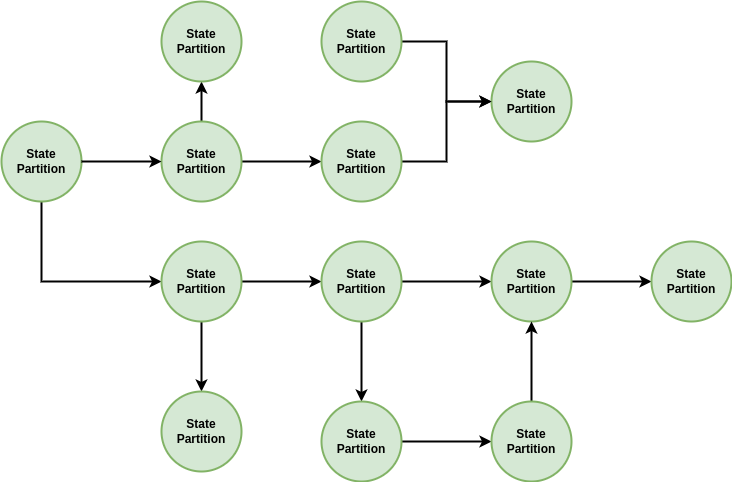
\includegraphics[width=12cm]{images/chapter-9-state-partition-graph.drawio.png}
\caption{State partition graph topology for multi-stage pipeline archetypes.}
\label{fig:state-partition-graph-multi-stage-pipelines}
\end{figure}

\textcolor{red}{
\begin{itemize}
\item{Talk about data}
\item{Logistics control papers}
\item{Data pipeline control papers}
\end{itemize}
}
